%\SweaveUTF8




\setkeys{Gin}{width=\textwidth}

\begin{Problem}[Weighing Basu's elephants]\label{problem:elephants}
    A circus owns 50 elephants.\footnote{This problem is adapted from Basu's
        famous elephant example in survey sampling; see Basu, D.
        (1971). An Essay on the Logical Foundations of Survey Sampling, Part 1,
        in: \emph{Foundations of Statistical Inference}. Proceedings of the
        Symposium on the Foundations of Statistical Inference Prepared Under
        the Auspices of the René Descartes Foundation and Held at the
        Department of Statistics, University of Waterloo, Ontario, Canada, from
        March 31 to April 9, 1970 ed. by Godambe, V. P. and Sprott, D. A.
        Toronto/ Montreal: Holt, Rinehart and Winston of Canada, pp. 203--233.
        The population data are taken from the book: Brewer, K. (2002),
        \emph{Combined Survey Sampling Inference: Weighing Basu's Elephants},
        London: Arnold, Appendix B.} The circus owner wants to estimate their
    total weight without having to weigh every elephant. He believes that Timbo
    is approximately as heavy as an average elephant and proposes weighing
    Timbo and multiplying his weight by 50, formally
    \begin{equation*}
        \tys^{\;\text{owner}} = 50 \cdot y_{\,\text{Timbo}}.
    \end{equation*}
    A statistician insists on probability sampling. They agree to select
    one elephant at random, with the following sampling design:
    \begin{equation*}
        p(s) = \begin{cases}
                0.99, & \qquad \text{if Timbo is selected},\\
                1/4900, & \qquad \text{otherwise}.
            \end{cases}
    \end{equation*}
    The statistician proposes using the Horvitz–Thompson estimator, $\tysht_y$,
    of the population total.

\begin{Subtask}
    %---------------------------------------------------------------------------
    \item Express the Horvitz–Thompson estimator in terms of the selected
        elephant's weight and its selection probability. Show that the
        estimator is design-unbiased.

    \begin{Solution}
        Let $I$ denote the index of the selected elephant. The HT estimator is
        \begin{equation*}
            \tysht_y = \begin{cases}
                \displaystyle{\frac{y_{\,\mathrm{Timbo}}}{0.99}}, &
                    \text{if Timbo is selected},\\[0.75em]
                4900 \cdot y_I, & \text{otherwise}.
            \end{cases}
        \end{equation*}
        Its design expectation is
        \begin{equation*}
            \EE\big(\,\tysht_y\big)
            = \sum_{i \in U} p(\{i\}) \frac{y_i}{p(\{i\})}
            = \sum_{i \in U} y_i = \ty.
        \end{equation*}
        Hence, the HT estimator is design-unbiased.
    \end{Solution}

    %---------------------------------------------------------------------------
    \item Suppose Timbo is selected and weighs 3\,900 kg. Calculate the
        estimates obtained by the circus owner and the statistician.
        Discuss the two estimates. Does design-unbiasedness guarantee that an
        estimator will give a reasonable estimate for the observed sample?

    \begin{Solution}
        Set

\begin{Schunk}
\begin{Sinput}
> y_timbo <- 3900
\end{Sinput}
\end{Schunk}

        The owner's estimator gives

\begin{Schunk}
\begin{Sinput}
> t_owner <- 50 * y_timbo
> t_owner
\end{Sinput}
\begin{Soutput}
[1] 195000
\end{Soutput}
\end{Schunk}

        whereas the HT estimator yields

\begin{Schunk}
\begin{Sinput}
> t_HT <- y_timbo / 0.99
> t_HT
\end{Sinput}
\begin{Soutput}
[1] 3939.394
\end{Soutput}
\end{Schunk}

        The estimates differ substantially. The owner's estimate is
        195\,000 kg, whereas the HT estimate is only about 3\,939 kg,
        roughly the weight of a single elephant.
        Design-unbiasedness does not guarantee an accurate estimate for
        a particular sample.

    \end{Solution}

    %---------------------------------------------------------------------------
    \item Ken Brewer provides the actual weights of all 50 elephants in the
        file:

\begin{Schunk}
\begin{Sinput}
> elephants <-
     read.table("https://stat.ethz.ch/Teaching/Datasets/cas-das/elephants.dat",
                header = TRUE)
\end{Sinput}
\end{Schunk}


        We can use these data to investigate the sampling distribution of the
        HT estimator. Construct the sampling distribution of the HT estimator
        by calculating its possible values and their probabilities. Also,
        calculate the design expectation and standard deviation of the HT
        estimator. Discuss the results.

    \begin{Solution}
        There are 50 possible samples, each consisting of one elephant. We
        calculate the sampling probabilities and the corresponding HT
        estimates.

\begin{Schunk}
\begin{Sinput}
> p <- ifelse(elephants$name == "Timbo", 0.99, 1/4900)
> t_HT <- elephants$weight / p
> sampling_dist <- data.frame(name = elephants$name, estimate = t_HT,
                              probability = p)
\end{Sinput}
\end{Schunk}

        The complete sampling distribution can be visualized by plotting the
        possible estimates against their probabilities; see Figure
        \ref{fig:ht_disr}. We use logarithmic scales because the estimates and
        probabilities differ substantially in magnitude.
        With probability 0.99, the estimator yields only about 3,939 kg. The
        remaining probability of 0.01 is distributed over extremely large
        estimates, ranging from approximately 12.7 to 29.0 million kg. These
        rare outcomes compensate for the severe underestimation when Timbo is
        selected.

\begin{Schunk}
\begin{Sinput}
> plot(t_HT, p, log = "xy", xlab = "HT estimate (kg, log)",
       ylab = "Sampling probability (log)")
> abline(v = sum(elephants$weight), lty = 2)
\end{Sinput}
\end{Schunk}

        \begin{figure}[tbp]
            \centering
            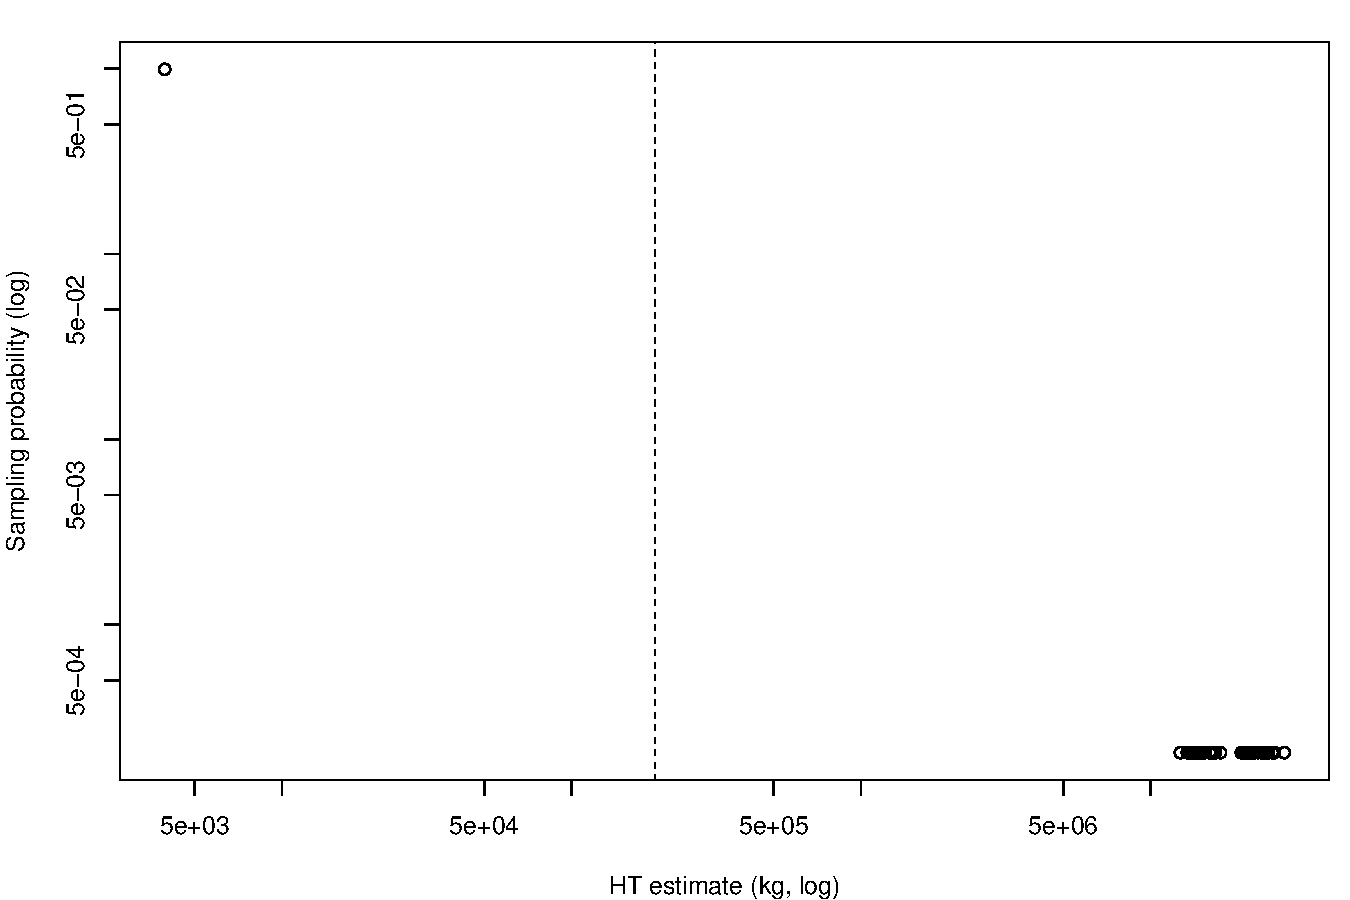
\includegraphics{problems/fig-ht_distr}
            \caption{Samplign distribution (axes in logarithmic scales; the
            dashed line shows the true population total)}
            \label{fig:ht_disr}
        \end{figure}

        The HT estimator is design-unbiased:

\begin{Schunk}
\begin{Sinput}
> E_HT <- sum(p * t_HT)
> identical(E_HT, as.numeric(sum(elephants$weight)))
\end{Sinput}
\begin{Soutput}
[1] TRUE
\end{Soutput}
\end{Schunk}

        The design standard deviation is approximately 1.95 million kg, about
        ten times the population total.

\begin{Schunk}
\begin{Sinput}
> SD_HT <- sqrt(sum(p * (t_HT - E_HT)^2))
> SD_HT
\end{Sinput}
\begin{Soutput}
[1] 1950266
\end{Soutput}
\end{Schunk}
    \end{Solution}
\end{Subtask}
\end{Problem}
